%!TEX root = ../main.tex

Στο παρών κεφάλαιο θα πραγματοποιηθεί μια αναλυτική παρουσίαση του θεωρητικού και τεχνολογικού υπόβαθρου, που αποτέλεσε βάση για την υλοποίηση της εφαρμογής. Αρχικά, θα δοθεί μια εξήγηση για το τι εστί απώλεια όρασης, τι δυσκολίες αντιμετωπίζουν τα άτομα με αυτό το είδος αναπηρίας, καθώς και τις τρέχουσες λύσεις για την καταπολέμηση δυσκολιών προσβασιμότητας (\hyperref[sec:visualImpairment]{Κεφάλαιο~\ref*{sec:visualImpairment}}). Στη συνέχεια, θα δοθεί ο ορισμός της εκτεταμένης πραγματικότητας, καθώς και τις εφαρμογές που βρίσκει στην καθημερινότητα του ανθρώπου (\hyperref[sec:extendedReality]{Κεφάλαιο~\ref*{sec:extendedReality}}). Τέλος, θα δοθεί μια περιγραφή της συσκευής Microsoft Hololens 2 και των λειτουργιών της (\hyperref[sec:hololensDesc]{Κεφάλαιο~\ref*{sec:hololensDesc}}), καθώς και τα εργαλεία, τα οποία θα χρησιμοποιηθούν για την ανάπτυξη της εφαρμογής (\hyperref[sec:hololensTools]{Κεφάλαιο~\ref*{sec:hololensTools}}).

\section{Όραση}\label{sec:visualImpairment}
\subsection{Τρόπος Λειτουργίας}\label{subsec:visionDefinition}
Η όραση αποτελεί μία από τις βασικές αισθήσεις του ανθρώπου. Η αίσθηση αυτή βασίζεται στη λειτουργία του ματιού, το οποίο αποτελεί το αισθητήριο όργανο και στο εσωτερικό του οποίου εισέρχεται το φως, διαπερνώντας αρχικά το κερατωειδή χιτώνα και την κόρη και προσπίπτει, τελικά, στον αμφιβληστροειδή χιτώνα (\hyperref[fig:eye_anatomy]{\schema~\ref*{fig:eye_anatomy}}). Αυτό οδηγεί σε διέγερση των οπτικών νεύρων και τα οπτικά σήματα, που αποστέλλονται στον εγκέφαλο, μετατρέπονται σε εικόνα~\cite{nationaleyeinstitute_2022_how}\cite{anspaugh_2022_vision}.

\begin{figure}[!h]
  \centering
  \includegraphics[width=90mm]{images/eye_anatomy.jpg}
  \caption[Η ανατομία του ματιού]{Η ανατομία του ματιού {\footnotesize(Πηγή: dreamstime.com)}}\label{fig:eye_anatomy}
\end{figure}

\subsection{Απώλεια Όρασης: Κατηγοροποίηση και Αιτίες}\label{subsec:visionCauses}
Όταν η φυσιολογική λειτουργία του αισθητήριου οργάνου διαταραχθεί, τότε το άτομο έρχεται αντιμέτωπο με κάποιο τύπο προβλήματος όρασης. Με βάση τον Παγκόσμιο Οργανισμό Υγείας (Π.Ο.Υ.), τα άτομα αυτά κατηγοροποιούνται σε 6 κατηγορίες (Κατηγορία 0 έως Κατηγορία 5), ανάλογα την οπτική τους οξύτητα, δηλαδή την ικανότητά τους να διακρίνουν σχήματα και λεπτομέρειες από κάποια δεδομένη απόσταση:
\begin{itemize}
    \item Στην κατηγορία 0 ανήκουν άτομα με με πλήρως ή σχεδόν πλήρως λειτουργική όραση
    \item Στην κατηγορία 1 και 2 ανήκουν άτομα που έχουν υποστεί μερική απώλεια της όρασής τους
    \item Τέλος, στις κατηγορίες 3, 4 και 5 εντάσσονται τα άτομα με σχεδόν πλήρη ή πλήρη απώλεια όρασης
\end{itemize}
Αντιθέτως, για κοντινές αποστάσεις, τα άτομα με προβλήματα όρασης εντάσσονται σε μία μόνο κατηγορία~\cite{worldhealthorganization_2019_world}.

Οι κυριότερες αιτίες, οι οποίες προκαλούν προβλήματα όρασης, αποτελούν:
\begin{itemize}
    \item τα διαθλαστικά σφάλματα
    \item ο καταρράκτης
    \item η διαβητική αμφιβληστροειδοπάθεια
    \item το γλαύκωμα
    \item η ηλικιακή εκφύλιση της ωχράς κηλίδας
\end{itemize}
Από τα ανωτέρω, η κυριότερη αίτια πλήρης απώλειας όρασης σε άτομα ηλικίας 50 ετών και άνω αποτελεί ο καταρράκτης, σε ποσοστό 46\% των ατόμων που υπέστησαν πλήρη απώλεια όρασης το 2020. Αντιθέτως, για την ίδια ηλικιακή ομάδα, η οποία αντιμετώπιζε μερική απώλεια όρασης, κύριες αιτίες αποτελούν τα υποδιορθωμένα διαθλαστικά σφάλματα και ο καταρράκτης, σε ποσοστό 30\% το καθένα για το ίδιο έτος~\cite{adelson_2021_causes}.

\subsection{Απώλεια Όρασης: Αντίκτυπος}\label{subsec:visionImpact}
Η απώλεια όρασης έχει ιδιαίτερο αντίκτυπο στην προσωπική, κοινωνική και οικονομική ζωή του ατόμου, ανεξάρτητα της ηλικίας του. Η εκπλήρωση απλών καθημερινών εργασιών μπορεί να αποδειχθεί ιδιαίτερα δύσκολη και χρονοβόρα, επιδεινώνοντας ιδιαίτερα την ποιότητα ζωής του ατόμου~\cite{west_2002_how}\cite{khorraminejad_2016_the}, ακόμη και σε επίπεδο χαμηλότερο από αυτό ατόμων που αντιμετωπίζουν χρόνια νοσήματα~\cite{langelaan_2007_impact}.



Η εμφάνιση προβλημάτων όρασης σε αρκετά νεαρή ηλικία μπορεί να επηρεάσει αισθητά την ανάπτυξη ικανοτήτων, όπως είναι η κινητήρια και η γνωστική ικανότητα και η κοινωνική καλλιέργεια~\cite{worldhealthorganization_2023_blindness}. Αντιθέτως, στην ενήλικη ζωή του ατόμου, μπορεί να δυσκολέψει την εύρεση εργασίας και να επηρεάσει την ψυχική του υγεία, προκαλώντας μέχρι και άγχος και κατάθλιψη~\cite{khorraminejad_2016_the}. Τέλος, σε άτομα αρκετά μεγάλης ηλικίας, η απώλεια όρασης μπορεί να αποτελέσει τροχοπέδη για βασικές λειτουργίες, όπως είναι το περπατήμα με εγγενές κίνδυνο την πτώση και τον τραυματισμό~\cite{worldhealthorganization_2023_blindness}.

\subsection{Απώλεια Όρασης: Λύσεις}\label{subsec:visionSolutions}
Πλήθος λύσεων είναι διαθέσιμες στο μέσο άνθρωπο, οι οποίες στοχεύουν στην πρόληψη της απώλειας της όρασης ή στην επιδιόρθωση αυτής. Σε απλές περιπττώσεις, όπως είναι η μυωπία, πρεσβυωπία, κ.λ.π., το πρόβλημα μπορεί να επιλυθεί με χρήση διορθωτικών φακών ή εγχείρηση στο αισθητήριο όργανο~\cite{worldhealthorganization_2023_blindness}. Επίσης, για άτομα που δεν μπορούν να επιδιορθώσουν το πρόβλημα όρασής τους, έχουν αναπτυχθεί συσκευές και τεχνολογίες, οι οποίες συνεχώς εξελίσσονται και έχουν ως σκοπό την εξυπηρέτηση του ατόμου σε διάφορες πτυχές της καθημερινότητάς του. Επί δεκαετείες, το μπαστούνι αποτελεί μια αρκετά διαδεδομένη συσκευή, που βοηθά ένα άτομο να αναγνωρίζει εμπόδια, καθώς περιηγείται σε έναν χώρο. Σε συνδυασμό με την απτική πλακόστρωση (\hyperref[fig:tactile_paving]{\schema~\ref*{fig:tactile_paving}}), το άτομο μπορεί να περιηγηθεί σε δημόσιο χώρο, όντας συνεχώς ενήμερο για την ύπαρξη εμποδίων, όπως δρόμοι, διάβαση πεζών, γραμμές τραμ, στη διαδρομή του, ανάλογα με το μοτίβο των πλακών του πεζοδρομίου~\cite{mashiata_2022_towards}.
\begin{figure}[!h]
  \centering
  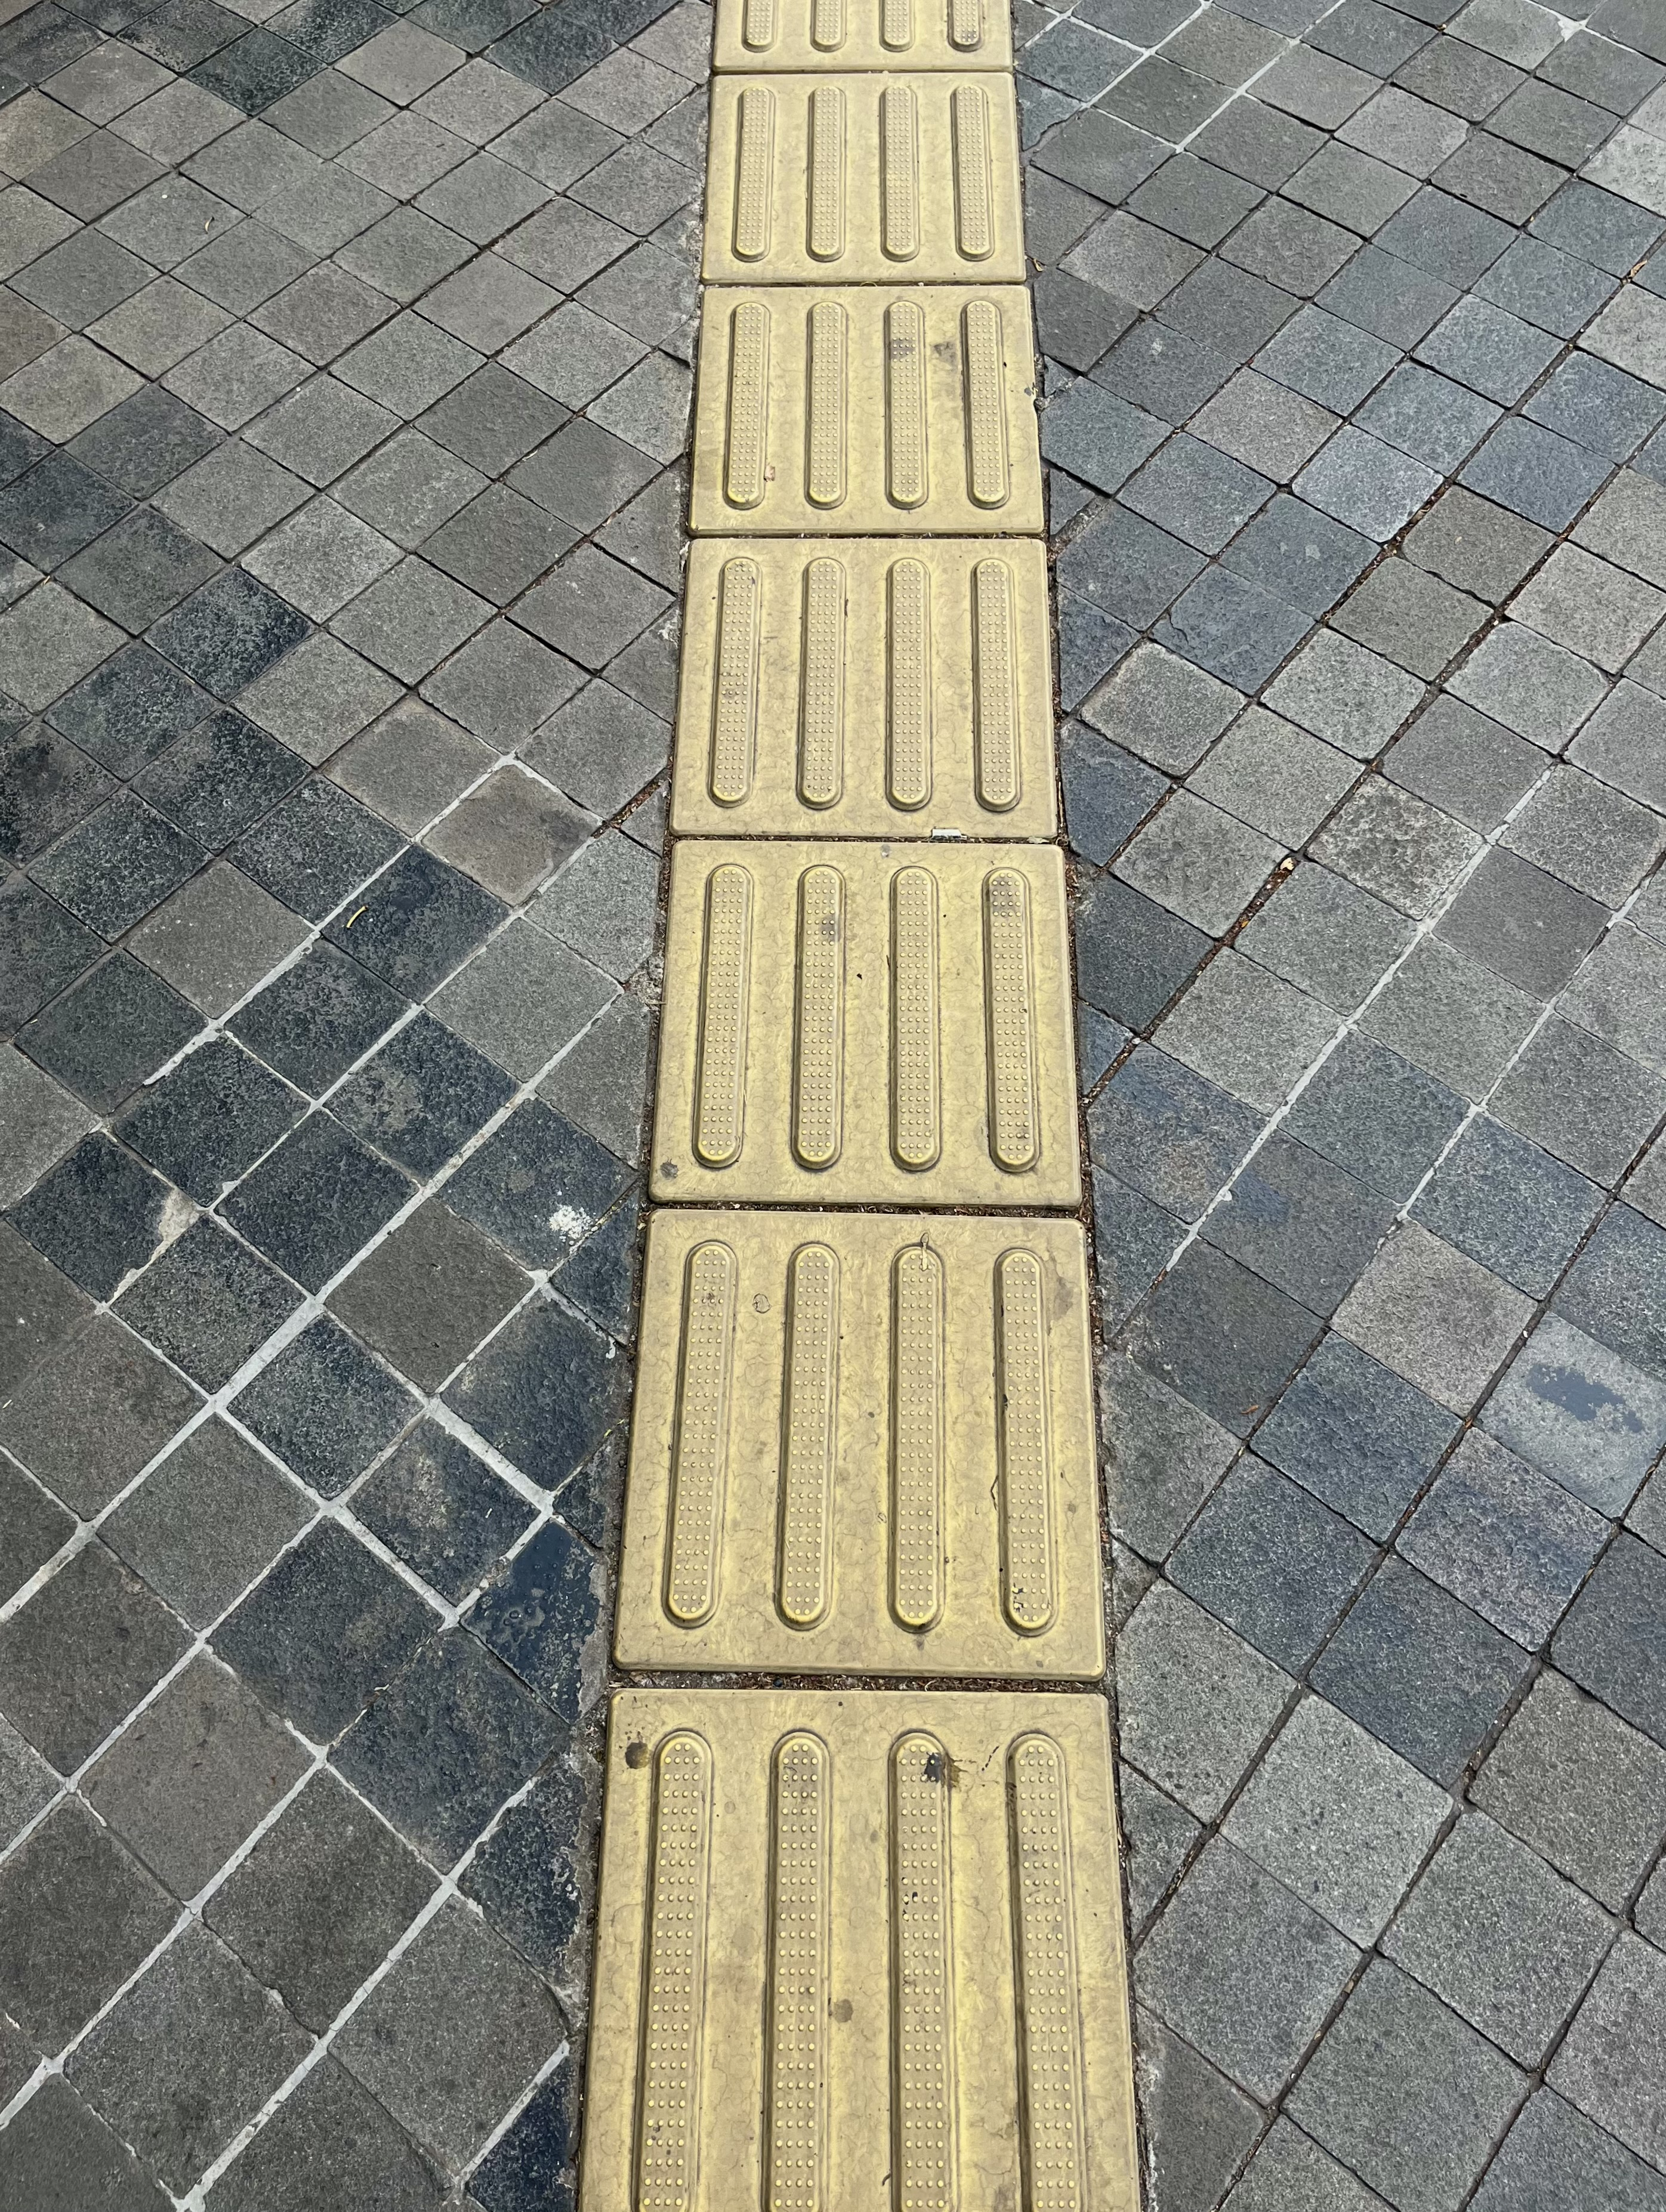
\includegraphics[width=60mm]{images/tactile-paving.jpg}
  \caption[Απτική πλακόστρωση]{Απτική πλακόστρωση {\footnotesize(Πηγή: vecteezy.com)}}\label{fig:tactile_paving}
\end{figure}\\
Ευρέως διαδεδομένη είναι και η χρήση σκύλων-βοηθών, οι οποίοι είναι ειδικά εκπαιδευμένοι σχετικά με την αναπηρία του ιδιοκτήτη τους με σκοπό να τους εξυπηρετήσουν στις ιδιαίτερες ανάγκες που μπορεί να έχουν. Στην περίπτωση των ατόμων με προβλήματα όρασης, σκοπός τους είναι να κατευθύνουν τον ιδιοκτήτη τους στο προορισμό του, ειδοποιώντας τον για πιθανά εμπόδια~\cite{illinoisuniversitylibrary_2013_libguides}. Τέλος, αναπτύχθηκε το σύστημα γραφής Braille, ώστε να είναι εφικτή η ανάγνωση κειμένων με τη βοήθεια της αφής.

Στη σύγχρονη εποχή, όλο και περισσότερες συσκευές κατασκευάζονται λαμβάνοντας εκ των προτέρων υπόψη τη δυνατότητα χρήσης αυτών από άτομα με περιορισμένη όραση. Οι κινητές συσκευές διαθέτουν λογισμικό screen reader (π.χ. TalkBack σε Android συσκεύες ή VoiceOver σε iOS συσκευές), διευκολύνοντας την πλοήγηση του χρήστη στις εφαρμογές του κινητού, καθώς πραγματοποιούν καταγραφή και αναγνώριση των κειμένων και των λειτουργιών, που βρίσκονται στην οθόνη τη δεδομένη χρονική στιγμή, και ο χρήστης, με συγκεκριμένες χειρονομίες, επιλέγει αν επιθυμεί την ανάγνωση κάποιου κειμένου με χρήση text-to-speech ή την πραγματοποίηση κάποιας ενέργειας~\cite{americanfoundationfortheblind_2019_screen}. Επιπλέον, η γλώσσα προγραμματισμού HTML δίνει τη δυνανότητα στους προγραμματιστές να κατασκευάσουν ιστοσελίδες, οι οποίες θα είναι προσβάσιμες από άτομα με περιορισμένη όραση, καθώς οι screen readers θα μπορούν να αναγνωρίζουν τμήματα της ιστοσελίδας, όπως επικεφαλίδες, υπερσυνδέσμους, κουμπιά και το σκοπό που επιτελούν~\cite{w3schools_2020_html}.

Όσον αφορά την περιήγηση ατόμων σε ανοιχτούς ή κλειστούς χώρους, πληθώρα συσκευών έχουν κατασκευαστεί, οι οποίες βελτιώνουν ήδη υπάρχουσες ή προσφέρουν έναν εναλλακτικό τρόπο λειτουργίας και παροχής βοήθειας. Παραδείγματα τέτοιων συσκευών αποτελούν:
\begin{itemize}
  \item \textbf{biped}: Συσκευή, η οποία φοριέται γύρω από το λαιμό του χρήστη. Διαθέτει 3 κάμερες, που προσφέρουν πεδίο ορατότητας 170\textdegree, και ενσωματώνουν λογισμικό για τον εντοπισμό και αναγνώριση εμποδίων. Ο χρήστης προειδοποιείται για εμπόδια με μια ηχητική προειδοποίηση.~\cite{biped}
  \item \textbf{OrCam MyEye}: Φορητή συσκευή, η οποία προσφέρει τη δυνατότητα ανάγνωσης κειμένων, αναγνώρισης αντικειμένων, χρωμάτων και προσώπων.~\cite{ghebali_2023_orcam}
  \item \textbf{BlindSquare}: Εφαρμογή πλοήγησης, η οποία παρέχει αναλύτικες\\οδηγίες στο χρήστη, ώστε να κατευθυνθεί στο προορισμό του, παρέχοντας παράλληλα πληροφορίες για το περιβάλλον του και για σημεία ενδιαφέροντος.~\cite{blindsquare}
  \item \textbf{Be My Eyes}: Εφαρμογή, η οποία επιτρέπει σε χρήστες να έρθουν σε επικοινωνία με εθελοντές μέσω βιντεοκλήσης, με σκοπό να ζητήσουν βοήθεια.~\cite{a2019_be}
  \item \textbf{WeWALK}: Αποτελεί ένα εξάρτημα για μπαστούνια, το οποίο έχει τη δυνατότητα να εντοπίζει εμπόδια σε χαμηλό ύψος με χρήση υπερήχων και να ειδοποιεί το χρήστη με δονήσεις και ήχο.~\cite{wewalk}
  \item \textbf{Seeing AI}: Εφαρμογή της Microsoft, η οποία, με χρήση τεχνητής νοημοσύνης, παρέχει περιγραφές των αντικειμένων, χρωμάτων, ανθρώπων και κειμένων, τα οποία στοχεύει ο χρήστης με την κάμερα του κινητού του τηλεφώνου.~\cite{seeing}
\end{itemize}

%=========================================

\section{Εκτεταμένη Πραγματικότητα}\label{sec:extendedReality}
% chktex-file 8

\tolerance=10000 Η εκτεταμένη πραγματικότητα (Extended Reality - XR) αποτελεί μια ιδιαιτέρως ευρεία έννοια, η οποία χρησιμοποιήθηκε πρώτη φορά το 1991 από τους Steve Mann και Charles Wyckoff, κατά την προσπάθεια κατασκευής συσκευών εικονικής/επαυξημένης πραγματικότητας~\cite{mann_2023_fundamentals}\cite{mann_1991_extended}. Αποτελεί `ομπρέλα' εννοιών και περιλαμβάνεις τις έννοιες της Εικονικής (Virtual Reality - VR, \hyperref[subsec:mixedReality]{Κεφάλαιο~\ref*{subsec:mixedReality}}), της Επαυξημένης (Augmented Reality - AR, \hyperref[subsec:augmentedReality]{Κεφάλαιο~\ref*{subsec:augmentedReality}}) και της Μικτής Πραγματικότητας (Mixed Reality - MR, \hyperref[subsec:mixedReality]{Κεφάλαιο~\ref*{subsec:mixedReality}})~\cite{milgram_1994_augmented}. To 1994, οι Paul Milgram και Fumio Kishino όρισαν ένα συνεχές μεταξύ πραγματικού και εικονικού κόσμου (\hyperref[fig:rv_continuum]{\schema~\ref*{fig:rv_continuum}}). Αυτοί οι δύο κόσμοι αποτελούν τα άκρα της κλίμακας και μεταξύ αυτών υπάρχουν οι έννοιες της επαυξημένης και μικτής πραγματικότητας, καθώς και της επαυξημένης εικονικότητας.
\begin{figure}[!h]
    \centering
    \includegraphics[width=120mm]{images/rv_continuum.png}
    \caption{Κλίμακα Πραγματικού Κόσμου - Εικονικού Κόσμου~\cite{milgram_1994_augmented}}\label{fig:rv_continuum}
\end{figure}

\subsection{Εικονική Πραγματικότητα}\label{subsec:virtualReality}
Η εικονική πραγματικότητα αποτελεί μια προσομοίωση, η οποία εντάσσει τον χρήστη σε έναν εικονικό κόσμο, κατασκευάσμενος από υπολογιστή, διεγείροντας αισθήσεις όπως η όραση (μπορεί να δει τον κόσμο αυτόν), η ακοή (μπορεί να ακούσει ήχους που προέρχονται από τον κόσμο αυτό) και η αφή (μπορεί να αντιληφθεί την επαφή με εικονικά αντικείμενα λαμβάνοντας απτική ανάδραση~\cite{weiler_2023_phantom}\cite{perret_2018_touching}), δίνοντάς του την δυνατότητα να αλληλεπιδράσει με αυτόν~\cite{lowood_2018_virtual}. Τα ανωτέρω επιτυγχάνονται με χρήση ειδικών συσκευών, όπως είναι τα γυαλιά εικονικής πραγματικότητας (VR headsets), τα οποία είτε ενσωματόνουν ειδικούς αισθητήρες με σκοπό να ανιχνεύσουν την κίνηση του κεφαλιού, είτε η ανίχνευση αυτή γίνεται με χρήση εξωτερικών αισθητήρων, που τοποθετούνται σε διάφορα σημεία στον περιβάλλοντα χώρο. Για την ανίχνευση της κίνησης των χέριων, που επιτρέπουν και την αλληλεπίδραση με εικονικά αντικείμενα, απαιτείται η χρήση χειριστηρίων. Παραδείγματα τέτοιων συσκευών αποτελούν το Meta Quest (\hyperref[fig:meta_quest_3]{\schema~\ref*{fig:meta_quest_3}}) και το Valve Index. Η VR τεχνολογία έχει εισβάλει πλέον και στην καθημερινότητα του μέσου χρήστη βρίσκοντας εφαρμογή σε ποικίλους τομείς:
\begin{itemize}
    \item Στην ψυχαγωγία και στη διασκέδαση, μέσω των βιντεοπαιχνιδιών που έχουν αναπτυχθεί, την δυνατότητα παρακολούθησης πραγματικών αθλητικών αγώνων, καθώς και εικονικών ξεναγήσεων σε χώρους πολιτιστικού ενδιαφέροντους~\cite{loeffler_1993_distributed}\cite{meta_2022_xtadium}\cite{ansari_2021_implementing}
    \item Στην εκπαίδευση, προσφέροντας έναν εναλλακτικό και διαδραστικό τρόπο εκμάθησης~\cite{hamad_2022_how}\cite{kavanagh_2017_a}\cite{freina_2015_a}
    \item Στην ιατρική, με σκοπό την εκπαίδευση και προετοιμασία ιατρών, καθώς και για να προσφέρει βοήθεια σε ασθενείς~\cite{chirico_2015_virtual}\cite{hamad_2022_how}\cite{snoswell_2019_immersive}\cite{gerup_2020_augmented}
\end{itemize}
\begin{figure}[!h]
    \centering
    \includegraphics[width=90mm]{images/meta_quest_3.jpg}
    \caption{Χρήστης φορά τα γυαλιά εικονικής πραγματικότητας Meta Quest 3}\label{fig:meta_quest_3}
\end{figure}

\subsection{Επαυξημένη Πραγματικότητα}\label{subsec:augmentedReality}
Η επαυξημένη πραγματικότητα αποτελεί μια τεχνολογία, η οποία `ενισχύει' τον πραγματικό κόσμο, ενσωματώνοντας τεχνητά δημιουργημένα, από υπολογιστή, στοιχεία (εικονικά αντικείμενα, ήχους) σε αυτόν. Τα στοιχεία αυτά βρίσκονται εντός ενός `στρώματος' (layer), το οποίο τοποθετείται `πάνω' από τον πραγματικό κόσμο, ο οποίος μπορεί να είναι μια φωτογραφία, ένα βίντεο ή ένα βίντεο πραγματικού χρόνου~\cite{hosch_2020_augmented}\cite{carmigniani_2011_augmented}. Λόγω της εξέλιξης των επεξεργαστών και την απλότητας της τεχνολογίας (σε σχέση με την εικονική πραγματικότητα), ένας χρήστη μπορεί να βιώσει την εμπειρία της επαυξημένης πραγματικότητας χρησιμοποιώντας μια απλή, έξυπνη κινητή συσκευή (smartphone)~\cite{ko_2013_usability}. Παράλληλα, είναι διαθέσιμα και γυαλιά επαυξημένης πραγματικότητας (AR headsets), όπως είναι τα Xreal Air AR Glasses και Magic Leap 2.

Η επαυξημένη πραγματικότητα βρίσκει εφαρμογή σε παρόμοιους τομείς με αυτούς της εικονικής πραγματικότητας:
\begin{itemize}
    \item Στην εκπαίδευση~\cite{wu_2013_current}\cite{lee_2012_augmented}
    \item Στον εργασιακό χώρο, αποτελώντας ένα επιπλέον εργαλείο για τον εργαζόμενο με σκοπό να διευκολύνει το έργο και να βελτιώσει την απόδοσή του~\cite{kim_2016_augmented}\cite{funk_2017_working}\cite{pereira_2023_augmented}
    \item Στην υγεία~\cite{klinker_2019_digital}\cite{zhu_2015_design}\cite{gerup_2020_augmented}\cite{solbiati_2020_augmented}
    \item Στην ψυχαγωγία~\cite{hung_2021_a}
    \item Στον τουρισμό, παρέχοντας ξεναγήσεις, όπου ο χρήστης μπορεί να μάθει περισσότερες πληροφορίες για μνημεία απλά στοχεύοντας την κάμερα του κινητού του σε αυτά~\cite{yovcheva_2012_smartphone}\cite{kounavis_2012_enhancing}
\end{itemize} 

\subsection{Μικτή Πραγματικότητα}\label{subsec:mixedReality}
Η `μικτή πραγματικότητα' αποτελεί μια εννοιά, η οποία, μέχρι και πρόσφατα, δεν έχει προσδιοριστεί ξεκαθάρα και επιδέχεται πληθώρα ορισμών, οι οποίοι, ωστόσο διαθέτουν μια κοινή βάση~\cite{speicher_2019_what}. Βάση του ορισμού που δόθηκε από τους Milgram και Kishino με το Συνεχές Πραγματικού-Εικονικού Κόσμου (\hyperref[fig:rv_continuum]{\schema~\ref*{fig:rv_continuum}}), η μικτή πραγματικότητα αποτελεί οτιδήποτε ανήκει μεταξύ των δύο άκρων της κλίμακας, όντας η επαυξημένη πραγματικότητα και η επαυξημένη εικονικότητα. Με τον όρο επαυξημένη εικονικότητα εννοείται ένας εικονικός κόσμος, στον οποίο ενσωματώνονται πραγματικά αντικείμενα του περιβάλλοντα χώρου~\cite{milgram_1994_augmented}. Ορισμένοι ακόμη δημοφιλείς ορισμοί της μικτής πραγματικότητας είναι:
\begin{enumerate}
    \item Η μικτή πραγματικότητα αποτελεί συνώνυμο της επαυξημένης πραγματικότητας
    \item Η τεχνολογίας μικτής πραγματικότητας αποτελεί μια ενισχημένη μορφή της τεχνολογίας επαυξημένης πραγματικότητας, όπου τα εικονικά αντικείμενα αλληλεπιδρούν με το πραγματικό περιβάλλον και τα αντικείμενα σε αυτόν
    \item Η μικτή πραγματικότητα αποτελεί συνδυασμός της επαυξημένης και της εικονικής πραγματικότητας, ενσωματώνοντας στοιχεία και από τις δύο τεχνολογίες
\end{enumerate}
Παράδειγμα συσκευών που αξιοποιούν την τεχνολογία μικτής πραγματικότητας αποτελούν τα Microsoft Hololens, Apple Vision Pro{\Large\footnotemark} και Meta Quest Pro.
Η μικτή πραματικότητα βρίσκει και αυτή ευρεία εφαρμογή σε αρκετούς τομείς της σύγχρονης καθημερινότητας, όπως είναι η εκπαίδευση~\cite{knierim_2018_challenges}\cite{liu_2007_mixed}, στην υγεία~\cite{chen_2017_recent}\cite{tepper_2017_mixed}, στην αρχιτεκτονική~\cite{wang_2008_mixed}\cite{dunston_2005_mixed} κ.α.

%=========================================

\section{Hololens}\label{sec:hololensDesc}

\subsection{Περιγραφή Συσκευής}
Description of the device

\subsection{Τεχνικά Χαρακτηριστικά}
Hololens features

\subsection{Τρόποι Αλληλεπίδρασης}
Τρόποι αλληλεπίδρασης

\subsection{Spatial Mapping}

\subsection{Spatial Audio}

%=========================================

\section{Εργαλεία ανάπτυξης για Hololens}\label{sec:hololensTools}

\subsection{Unity}
Περιγραφή περιβάλλοντος

\subsection{Microsoft Visual Studio}
Μικρή περιγραφή της χρήσης του

\subsection{Mixed Reality Toolkit}

%=========================================